\section{Date: 2026-08-12}
\noindent \textbf{Series ID: CHINTDUSDDM} 

\noindent This series is titled Swiss Intervention: Swiss National Bank Purchases of USD against DEM (Millions of USD) and has a frequency of Daily, 7-Day. The units are Millions of USD and the seasonal adjustment is Not Seasonally Adjusted.The observation start date is 1975-01-01 and the observation end date is 1998-12-31.The popularity of this series is 2. \\ 

\noindent \textbf{Series ID: U36SUS} 

\noindent This series is titled Manufacturers' Unfilled Orders to Shipments Ratios: Transportation Equipment and has a frequency of Monthly. The units are Ratio and the seasonal adjustment is Not Seasonally Adjusted.The observation start date is 1992-01-01 and the observation end date is 2026-06-01.The popularity of this series is 1. \\ 

\subsection{Raw Regression}
\noindent Regresses the two series against each other directly. A significant result here can come just as easily from both series sharing a long-run trend as from any real relationship.

\begin{center}
\begin{tabular}{lclc}
\toprule
\textbf{Dep. Variable:}           & value\_fred\_U36SUS & \textbf{  R-squared:         } &     0.000   \\
\textbf{Model:}                   &         OLS         & \textbf{  Adj. R-squared:    } &     0.000   \\
\textbf{Method:}                  &    Least Squares    & \textbf{  F-statistic:       } &       nan   \\
\textbf{Date:}                    &   Wed, 12 Aug 2026  & \textbf{  Prob (F-statistic):} &      nan    \\
\textbf{Time:}                    &       12:39:50      & \textbf{  Log-Likelihood:    } &   -151.34   \\
\textbf{No. Observations:}        &            84       & \textbf{  AIC:               } &     304.7   \\
\textbf{Df Residuals:}            &            83       & \textbf{  BIC:               } &     307.1   \\
\textbf{Df Model:}                &             0       & \textbf{                     } &             \\
\textbf{Covariance Type:}         &      nonrobust      & \textbf{                     } &             \\
\bottomrule
\end{tabular}
\begin{tabular}{lcccccc}
                                  & \textbf{coef} & \textbf{std err} & \textbf{t} & \textbf{P$> |$t$|$} & \textbf{[0.025} & \textbf{0.975]}  \\
\midrule
\textbf{const}                    &       9.3852  &        0.161     &    58.316  &         0.000        &        9.065    &        9.705     \\
\textbf{value\_fred\_CHINTDUSDDM} &            0  &            0     &       nan  &           nan        &            0    &            0     \\
\bottomrule
\end{tabular}
\begin{tabular}{lclc}
\textbf{Omnibus:}       & 19.125 & \textbf{  Durbin-Watson:     } &    1.105  \\
\textbf{Prob(Omnibus):} &  0.000 & \textbf{  Jarque-Bera (JB):  } &   23.295  \\
\textbf{Skew:}          &  1.168 & \textbf{  Prob(JB):          } & 8.74e-06  \\
\textbf{Kurtosis:}      &  4.095 & \textbf{  Cond. No.          } &      inf  \\
\bottomrule
\end{tabular}
%\caption{OLS Regression Results}
\end{center}

Notes: \newline
 [1] Standard Errors assume that the covariance matrix of the errors is correctly specified. \newline
 [2] The smallest eigenvalue is      0. This might indicate that there are \newline
 strong multicollinearity problems or that the design matrix is singular.

\begin{figure}
\centering
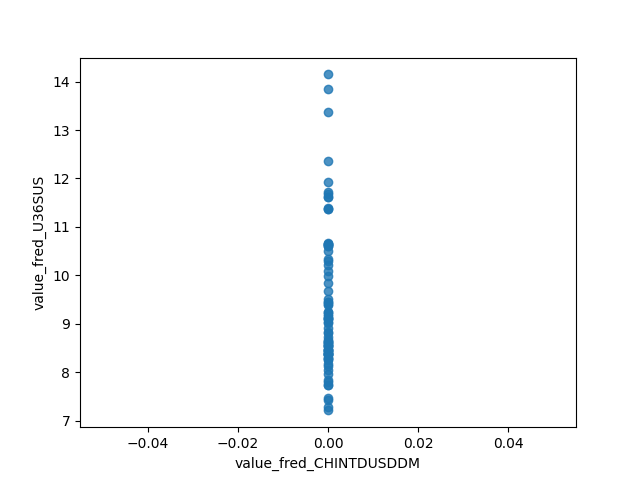
\includegraphics[scale = 0.9]{plots/plot_2026-08-12.png}
\caption{Raw Regression Plot for 2026-08-12}
\end{figure}
\newpage
\subsection{Detrended Regression}
\noindent Regresses the residuals of each series after removing its own linear time trend, so a shared trend can no longer drive the result on its own. A relationship that stays significant here is better evidence of a genuine link between the two series.

\begin{center}
\begin{tabular}{lclc}
\toprule
\textbf{Dep. Variable:}                      & value\_fred\_U36SUS\_detrended & \textbf{  R-squared:         } &     0.000   \\
\textbf{Model:}                              &              OLS               & \textbf{  Adj. R-squared:    } &     0.000   \\
\textbf{Method:}                             &         Least Squares          & \textbf{  F-statistic:       } &       nan   \\
\textbf{Date:}                               &        Wed, 12 Aug 2026        & \textbf{  Prob (F-statistic):} &      nan    \\
\textbf{Time:}                               &            12:39:50            & \textbf{  Log-Likelihood:    } &   -134.10   \\
\textbf{No. Observations:}                   &                 84             & \textbf{  AIC:               } &     270.2   \\
\textbf{Df Residuals:}                       &                 83             & \textbf{  BIC:               } &     272.6   \\
\textbf{Df Model:}                           &                  0             & \textbf{                     } &             \\
\textbf{Covariance Type:}                    &           nonrobust            & \textbf{                     } &             \\
\bottomrule
\end{tabular}
\begin{tabular}{lcccccc}
                                             & \textbf{coef} & \textbf{std err} & \textbf{t} & \textbf{P$> |$t$|$} & \textbf{[0.025} & \textbf{0.975]}  \\
\midrule
\textbf{const}                               &    -8.19e-13  &        0.131     & -6.25e-12  &         1.000        &       -0.261    &        0.261     \\
\textbf{value\_fred\_CHINTDUSDDM\_detrended} &            0  &            0     &       nan  &           nan        &            0    &            0     \\
\bottomrule
\end{tabular}
\begin{tabular}{lclc}
\textbf{Omnibus:}       & 21.603 & \textbf{  Durbin-Watson:     } &    1.662  \\
\textbf{Prob(Omnibus):} &  0.000 & \textbf{  Jarque-Bera (JB):  } &   27.747  \\
\textbf{Skew:}          &  1.266 & \textbf{  Prob(JB):          } & 9.44e-07  \\
\textbf{Kurtosis:}      &  4.233 & \textbf{  Cond. No.          } &      inf  \\
\bottomrule
\end{tabular}
%\caption{OLS Regression Results}
\end{center}

Notes: \newline
 [1] Standard Errors assume that the covariance matrix of the errors is correctly specified. \newline
 [2] The smallest eigenvalue is      0. This might indicate that there are \newline
 strong multicollinearity problems or that the design matrix is singular.

\begin{figure}
\centering
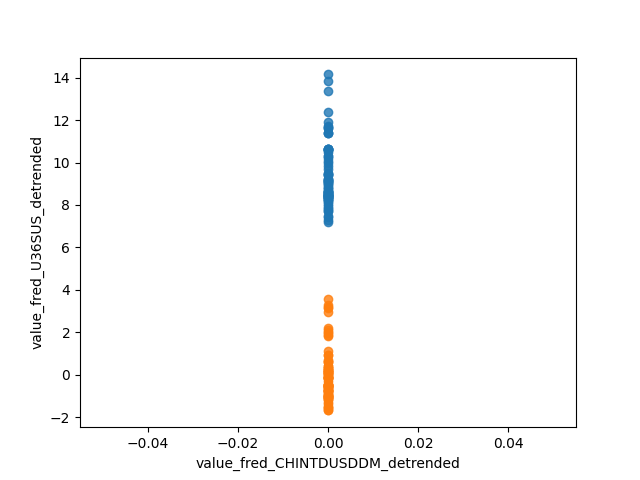
\includegraphics[scale = 0.9]{plots/plot_2026-08-12_detrended.png}
\caption{Detrended Regression Plot for 2026-08-12}
\end{figure}
\newpage
